\section{Durchführung}
\label{sec:Durchführung}
\begin{figure}
  \centering
  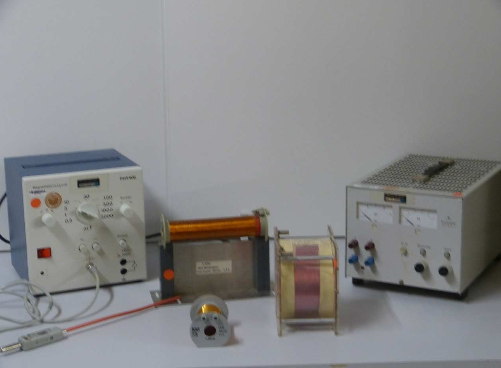
\includegraphics[width=0.5\textwidth]{content/images/aufbau1.png}
  \caption{Aufbau zur Messung einer Einzelspule.\cite{anleitung}.}
  \label{fig:a1}
\end{figure}
\begin{figure}
  \centering
  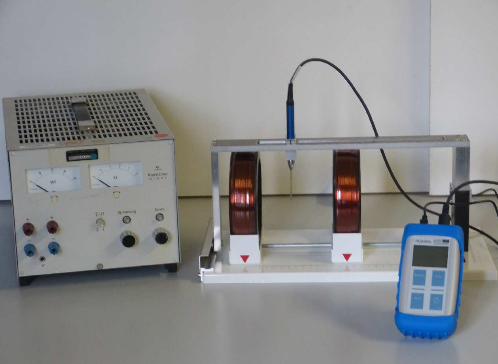
\includegraphics[width=0.5\textwidth]{content/images/aufbau2.png}
  \caption{Aufbau zur Messung der Helmholzspule.\cite{anleitung}.}
  \label{fig:a2}
\end{figure}
\begin{figure}
  \centering
  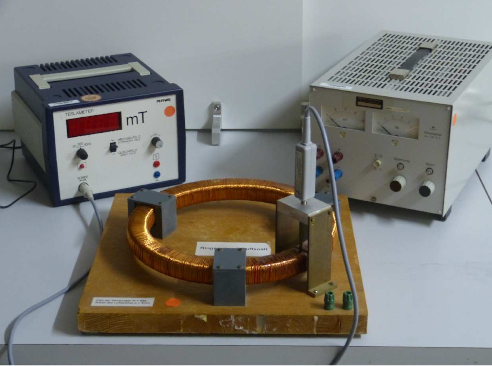
\includegraphics[width=0.5\textwidth]{content/images/aufbau3.png}
  \caption{Aufbau zur Messung der Hysteresekurve.\cite{anleitung}.}
  \label{fig:a3}
\end{figure}
